\documentclass[11pt]{article}
%\documentclass[11pt]{book}
%\documentclass[12pt]{report}
%\documentclass[12pt,a4paper,oneside]{book}
%\documentclass[12pt,a4paper,twoside]{book}

\usepackage[italian]{babel} % per la sillabazione in italiano
\usepackage[utf8]{inputenc} %e per usare tutti i simboli nella tastiera


\usepackage{ theorem}  % uso questo e il seguente in alternativa a \usepackage{amsthm} 
\newenvironment{proof}{\noindent{\bf Proof:\/}}{$\Box$\vskip 0.1in}

\usepackage{ amsfonts}
\usepackage{amscd}
\usepackage{amssymb}
\usepackage{amsmath}
\usepackage{bm,bbm}
\usepackage{amsbsy}
\usepackage{mathrsfs}
\usepackage{fancyhdr}
%\usepackage{amsthm} 
%in genere si mettono sempre quando si scrive matematica... arricchiscono la scelta per le formule

\usepackage{latexsym}
\usepackage{makeidx} %compila gli indici analitici
\usepackage{graphicx} %facilita la gestione delle figure
%\usepackage[a-1b]{pdfx} %cerca di adattare il pdf alle specifiche del formato archiviabile PDF-A

 




 % SIDE MARGINS:
\oddsidemargin 0cm      %   Left margin on odd-numbered pages.
 \evensidemargin 0cm     %   Left margin on even-numbered pages.
 \marginparwidth 40pt    %   Width of marginal notes.
 \marginparsep 10pt      %   Horizontal space between outer margin and
             %   marginal note


 % VERTICAL SPACING:
 \topmargin 0cm           %    Nominal distance from top of page to top of
              %    box containing running head.
 \headsep 10pt            %    Space between running head and text.

 % DIMENSION OF TEXT:
 \textheight 23.0cm       % Height of text (including footnotes and figures,
              % excluding running head and foot).

 \textwidth 16.0cm        % Width of text line.
\baselineskip 0.8cm


 \setcounter{page}{0}     % First page number starts from 0

  \newtheorem{defin}{Definizione}[section]
  \newtheorem{prop}{Proposizione}[section]
  \newtheorem{lemma}{Lemma}[section]
  \newtheorem{coro}{Corollario}[section]
  \newtheorem{theorem}{Teorema}
  \newtheorem{fatto}{Fatto}[section]
  \newtheorem{open-probl}{Problema aperto}[section]
  \newtheorem{esem}{Esempio}[section]


\newcommand{\R}{\mathbb{R}}
\newcommand{\N}{\mathbb{N}}


\title{ { \bf Terza lezione del corso di \LaTeX } \thanks{Si prega di segnalare eventuali errori all'autore}}

\author{
   \Large{Dora Giammarresi}\\ \emph {Dipartimento di Matematica.
   Università di Roma ``Tor Vergata''}\\
   via della Ricerca Scientifica, 00133 Roma, Italy. \\ E-mail:{\tt giammarr@mat.uniroma2.it}
}

\date{12 novmbre 2019} %senza il comando \date viene generata la data corrente
                % con il comando vuoto \date{} non viene messa alcuna data

\begin{document}

\maketitle %genera il titolo con autore e data


\section{Introduzione}\label{s-intro}

Nella Sezione \ref{s-preli} saranno introdotte tutte le notazioni utilizzate per illustrare i teoremi della Sezione \ref{s-main}.
In particolare le Sezioni \ref{s-fin} e \ref{s-infin} tratteranno rispettivamente il caso in cui l'insieme di partenza sia rispettivamente finito o infinito.
Tutte le conseguenze dei teoremi sulla teoria generale saranno discusse nella Sezione \ref{s-conclu}.


\section{Notazioni e definizioni preliminari}\label{s-preli}

\begin{equation}\label{eq-defsim}
\forall n\in \N ,  a^n=b^{n+3}
\end{equation}

\begin{equation*}
\begin{pmatrix}
a_{11} & a_{12} & \dots & a_{1n} \\
a_{21} & a_{22} & \dots & a_{2n} \\
\vdots & \vdots & \ddots & \vdots \\
a_{n1} & a_{n2} & \dots & a_{nn}
\end{pmatrix}
\end{equation*}


\begin{equation*}
\begin{bmatrix} 1 & 2 \\ 3 & 4
\end{bmatrix} \quad
\begin{vmatrix} 1-x & 2 \\ 3 & 4-x
\end{vmatrix}
\end{equation*}

\begin{equation*}
\begin{Bmatrix} 1 & 2 \\ 3 & 4
\end{Bmatrix} \quad
\begin{Vmatrix} 1-x & 2 \\ 3 & 4-x
\end{Vmatrix}
\end{equation*}

\section{Risultati principali}\label{s-main}
\begin{defin}\label{d-mat}
Due matrici $n \times n$ complesse
$A=
\begin{array}{ccc}
   a_{11} &  a_{12} &  a_{13} \\
   a_{21} &  a_{22} &  a_{23} \\
   a_{31} &  a_{32} &  a_{33} \\
\end{array}$
e $B=\left(
       \begin{array}{ccc}
         b_{11} &  b_{12} &  b_{13} \\
   b_{21} &  b_{22} &  b_{23} \\
   b_{31} &  b_{32} &  b_{33} \\
       \end{array}
     \right)
$
si dicono \emph{simili}
se esiste una matrice $n \times n$
invertibile $T$ tale che
$
B=T^{-1}AT
$
\end{defin}

Se sappiamo risolvere il seguente sistema di equazioni:
\begin{equation}\label{e-sist}
\left\{
\begin{array}{l}
x+y+z=0\\ 
2x-y=1\\
y-4z=-3
\end{array}
\right.
\end{equation} 

\begin{theorem}\label{t-pit}
In un triangolo rettangolo il quadrato costruito sull'ipotenusa è uguale alla somma dei quadrati costruiti sui cateti.
\end{theorem}

\begin{proof}
Si consideri un triangolo strano i cui lati soddisfano il sistema di equazioni in \ref{e-sist}. Cosa possiamo dire?

\end{proof}

\begin{figure}
\begin{center}
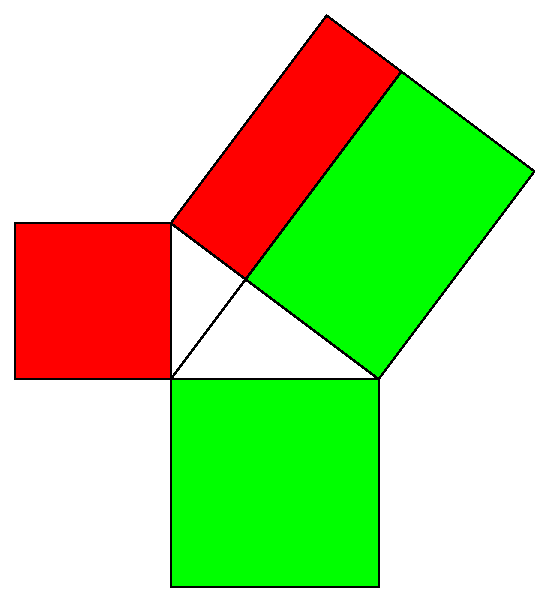
\includegraphics{pitagora}
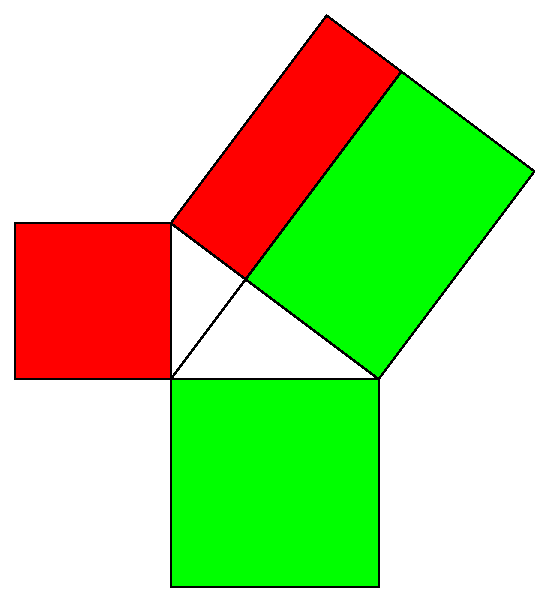
\includegraphics[width=.4\textwidth]{pitagora}
\caption{Teorema di
Pitagora}
\label{pitagora}
\end{center}
\end{figure}

\subsection{Caso finito}\label{s-fin}
Il Teorema \ref{t-pit} vale anche ...

\subsection{Caso infinito}\label{s-infin}

\section{Conclusioni}\label{s-conclu}




\end{document}
